\documentclass[twoside]{article}
\setlength{\oddsidemargin}{0.25 in}
\setlength{\evensidemargin}{-0.25 in}
\setlength{\topmargin}{-0.6 in}
\setlength{\textwidth}{6.5 in}
\setlength{\textheight}{8.5 in}
\setlength{\headsep}{0.75 in}
\setlength{\parindent}{0 in}
\setlength{\parskip}{0.1 in}
\newcommand{\eqdef}{:\mathrel{\mathop=}}
\newcommand{\norm}[1]{\left\lVert #1 \right\rVert}

%
% ADD PACKAGES here:
%

\usepackage{amsmath,amsfonts,graphicx,dsfont,amssymb, cool, cancel, mathtools}
%
% The following commands set up the lecnum (lecture number)
% counter and make various numbering schemes work relative
% to the lecture number.
%
\newcounter{lecnum}
\renewcommand{\thepage}{\thelecnum-\arabic{page}}
\renewcommand{\thesection}{\thelecnum.\arabic{section}}
\renewcommand{\theequation}{\thelecnum.\arabic{equation}}
\renewcommand{\thefigure}{\thelecnum.\arabic{figure}}
\renewcommand{\thetable}{\thelecnum.\arabic{table}}
\newcommand{\indep}{\raisebox{0.05em}{\rotatebox[origin=c]{90}{$\models$}}}

%
% The following macro is used to generate the header.
%
\newcommand{\lecture}[4]{
   \pagestyle{myheadings}
   \thispagestyle{plain}
   \newpage
   \setcounter{lecnum}{#1}
   \setcounter{page}{1}
   \noindent
   \begin{center}
   \framebox{
      \vbox{\vspace{2mm}
    \hbox to 6.28in { {\bf Advanced Machine Learning
	\hfill Fall 2020} }
       \vspace{4mm}
       \hbox to 6.28in { {\Large \hfill Lecture #1: #2  \hfill} }
       \vspace{2mm}
       \hbox to 6.28in { {\it  #3 \hfill  #4} }
      \vspace{2mm}}
   }
   \end{center}
   \markboth{Lecture #1: #2}{Lecture #1: #2}

   {\bf Note}: {\it LaTeX template courtesy of UC Berkeley EECS dept.}

   {\bf Disclaimer}: {\it These notes are adapted from ETH's Advanced Machine Learning Course, "Gaussian Processes for Machine Learning, the MIT Press", "Probabilistic Machine Learning: An introduction, MIT Press" and MA4270 Lecture Notes 5.}
   \vspace*{4mm}
}
%
% Convention for citations is authors' initials followed by the year.
% For example, to cite a paper by Leighton and Maggs you would type
% \cite{LM89}, and to cite a paper by Strassen you would type \cite{S69}.
% (To avoid bibliography problems, for now we redefine the \cite command.)
% Also commands that create a suitable format for the reference list.
\renewcommand{\cite}[1]{[#1]}
\def\beginrefs{\begin{list}%
        {[\arabic{equation}]}{\usecounter{equation}
         \setlength{\leftmargin}{2.0truecm}\setlength{\labelsep}{0.4truecm}%
         \setlength{\labelwidth}{1.6truecm}}}
\def\endrefs{\end{list}}
\def\bibentry#1{\item[\hbox{[#1]}]}

%Use this command for a figure; it puts a figure in wherever you want it.
%usage: \fig{NUMBER}{SPACE-IN-INCHES}{CAPTION}
\newcommand{\fig}[3]{
			\vspace{#2}
			\begin{center}
			Figure \thelecnum.#1:~#3
			\end{center}
	}
% Use these for theorems, lemmas, proofs, etc.
\newtheorem{theorem}{Theorem}[lecnum]
\newtheorem{lemma}[theorem]{Lemma}
\newtheorem{proposition}[theorem]{Proposition}
\newtheorem{claim}[theorem]{Claim}
\newtheorem{corollary}[theorem]{Corollary}
\newtheorem{definition}[theorem]{Definition}
\newenvironment{proof}{{\bf Proof:}}{\hfill\rule{2mm}{2mm}}

% **** IF YOU WANT TO DEFINE ADDITIONAL MACROS FOR YOURSELF, PUT THEM HERE:

\DeclareMathOperator*{\argmax}{arg\,max} 
\DeclareMathOperator*{\argmin}{arg\,min} 

\begin{document}
%FILL IN THE RIGHT INFO.
%\lecture{**LECTURE-NUMBER**}{**DATE**}{**LECTURER**}{**SCRIBE**}
\lecture{5}{Gaussian Processes}{}{}
%\footnotetext{These notes are partially based on those of Nigel Mansell.}

% **** YOUR NOTES GO HERE:

% Some general latex examples and examples making use of the
% macros follow.  
%**** IN GENERAL, BE BRIEF. LONG SCRIBE NOTES, NO MATTER HOW WELL WRITTEN,
%**** ARE NEVER READ BY ANYBODY.

\section{Kernel Methods}

In the previous lecture we have looked at \textit{linear predictors} for real-valued variables of the form:
\begin{equation*}
      \hat{y} = \hat{f}(\boldsymbol{x}, \boldsymbol{\theta}) = \theta_0 +  \boldsymbol{\theta}^\intercal\boldsymbol{x}
\end{equation*}
\textit{Motivation example (Fitting a quadratic):} If we know that $y$ is (well-approximated by) a quadratic function of a single input $\boldsymbol{x}$, then we can use $\boldsymbol{x}$ to construct $\Tilde{\boldsymbol{x}} = [x, x^2]^\intercal$, and then perform linear regression with input $\Tilde{\boldsymbol{x}}$ and $\boldsymbol{\theta} \in \mathbb{R}^2$. Then $\hat{y} = \theta_2x^2 + \theta_1x + \theta_0$, an arbitrary quadratic function.\medskip

\textbf{Overview}
\begin{itemize}
    \item Many machine learning algorithms depend on the data $x_1,...,x_n$ only through products $\langle x_i, x_j \rangle$.\\
    Inner products capture the geometry of the data set, so one generally expects geometrically inspired algorithms (e.g. SVM) to depend only on inner products. For algorithms that use distances, note that $\norm{\boldsymbol{x} - \boldsymbol{x'}}^2 = \langle \boldsymbol{x}, \boldsymbol{x} \rangle + \langle \boldsymbol{x'}, \boldsymbol{x'} \rangle - 2\langle \boldsymbol{x}, \boldsymbol{x'} \rangle$, so distances can be expressed in terms of inner products.
    \item We know that moving to feature spaces can help, so we could map each $x_i \rightarrow \phi(x_i)$ and apply the algorithm using $\langle \phi(x_i), \phi(x_j) \rangle$.
    \item A \textit{kernel function} $k(x_i, x_j)$ can be thought of as an inner product in a \textit{possibly implicit} feature space:
    \begin{itemize}
        \item \textbf{Key idea}: There are clever choices of the mapping $\phi(\cdot)$  ensuring that we can efficiently compute $\langle \phi(x_i), \phi(x_j) \rangle$ without ever explicitly mapping to the feature space.
        \item In some cases, the feature space is infinite-dimensional, so we could not explicitly map to it even if we wanted to.
    \end{itemize}
    \item \textbf{Kernel trick}: The terminology “kernel trick” simply refers to taking any algorithm the depends on the data only through inner products, and replacing each inner product $\langle \boldsymbol{x}, \boldsymbol{x'} \rangle$ by a kernel value $k(\boldsymbol{x}, \boldsymbol{x'})$.
\end{itemize}\medskip

\begin{definition}
A function $k : \mathbb{R}^d \times \mathbb{R}^d \rightarrow \mathbb{R}$ is said to be a kernel function if and only if it is an inner product $\langle \boldsymbol{\phi(x)}, \boldsymbol{\phi(x')} \rangle$  for some (possibly infinite dimensional) mapping $\boldsymbol{\phi(x)}$.
\end{definition}
\newpage
\begin{definition}
A function $k : \mathbb{R}^d \times \mathbb{R}^d \rightarrow \mathbb{R}$ is said to be symmetric positive semidefinite (PSD) if it is symmetric, i.e \: $k(\boldsymbol{x}, \boldsymbol{x'}) = k(\boldsymbol{x'}, \boldsymbol{x})$; For any integer $m > 0$ and any set of inputs $\boldsymbol{x_1,...,x_m }\in \mathbb{R}^d$, the following matrix is positive semi-definite:
\begin{center}
    $\boldsymbol{K} =
    \begin{bmatrix}
    k(\boldsymbol{x_1}, \boldsymbol{x_1}) & \hdots & k(\boldsymbol{x_1}, \boldsymbol{x_m})\\
    \vdots & \ddots & \vdots\\
    k(\boldsymbol{x_m}, \boldsymbol{x_1}) & \hdots & k(\boldsymbol{x_m}, \boldsymbol{x_m})
    \end{bmatrix}
    \succeq \boldsymbol{0}
$
\end{center}
This matrix, with $(i, j)$-th entry equal to $k(\boldsymbol{x_i}, \boldsymbol{x_j})$, is called the \textbf{Gram matrix}.
\end{definition}

\begin{theorem}
Two above two definitions are equivalent. That is, $k$ is a kernel function if and only if it is symmetric PSD.
\end{theorem}
\begin{proof}
The “only if” part is easy to show (at least when $\phi$ is finite-dimensional): The inner product is certainly symmetric, and the Gram matrix can be written as $\boldsymbol{K = \Phi^\intercal\Phi}$, where $\boldsymbol{\Phi} \in \mathbb{R}^{\text{dim}(\boldsymbol{\Phi}) \times m}$ contains the $m$ feature vectors $\{\boldsymbol{\phi(x_t)}\}_{t = 1}^{m}$ as columns. The matrix $\boldsymbol{K = \Phi^\intercal\Phi}$  is trivially positive semidefinite, since for any $\boldsymbol{z}$ we have $\boldsymbol{z^\intercal\Phi^\intercal\Phi z} = \boldsymbol{\norm{\Phi z}^2} \geq 0$.\medskip

The “if” part is more challenging and comes from \textit{Mercer's Theorem}.
\end{proof}\medskip

\begin{theorem}{\textbf{Mercer's  Theorem}\\}
Recall: any positive definite matrix $\boldsymbol{K}$ can be represented using an eigendecomposition of the form $\boldsymbol{K = U^\intercal\Lambda U}$, where $\boldsymbol{\Lambda}$ is a diagonal matrix of eigenvalues $\lambda_i > 0$, and $\boldsymbol{U}$ is a matrix containing the eigenvectors.\\
Now consider element $(i, j)$ of $\boldsymbol{K}$:
\begin{equation*}
    k_{ij} = (\boldsymbol{\Lambda}^\frac{1}{2}\boldsymbol{U}_{:i})^\intercal(\boldsymbol{\Lambda}^\frac{1}{2}\boldsymbol{U}_{:j})
\end{equation*}
where $\boldsymbol{U}_{:i}$ is the \textit{i}'th column of $\boldsymbol{U}$. If we define $\boldsymbol{\phi(x_i)} = \boldsymbol{\Lambda}^\frac{1}{2}\boldsymbol{U}_{:i}$, then we can write:
\begin{equation*}
    k_{ij} = \boldsymbol{\phi(x_i)}^\intercal \boldsymbol{\phi(x_j)} = \sum\limits_m \phi_m (\boldsymbol{x_i})\phi_m(\boldsymbol{x_j})
\end{equation*}
\end{theorem}
Thus we see that the entries in the kernel matrix can be computed by performing an inner product of some feature vectors that are implicitly defined by the eigenvectors of the kernel matrix. This idea can be generalized to apply to kernel functions, not just kernel matrices.\\
For example consider the \textbf{quadratic kernel} $\mathcal{K}(\boldsymbol{x}, \boldsymbol{x'}) = \langle\boldsymbol{x}, \boldsymbol{x'}\rangle^2$. In 2d, we have:
\begin{equation*}
    \mathcal{K}(\boldsymbol{x}, \boldsymbol{x'}) = (x_1x_1' + x_2x_2')^2 = x_1^2(x_1')^2 + 2x_1x_2x_1'x_2' + x_2^2(x_2')^2
\end{equation*}
We can write this as $\mathcal{K}(\boldsymbol{x}, \boldsymbol{x'}) = \boldsymbol{\phi(x)}^\intercal\boldsymbol{\phi(x)}$ if we define $\boldsymbol{\phi(x_1, x_2)} = [x_1^2, \sqrt{2}x_1x_2, x_2^2] \in \mathbb{R}^3$. So we embed the 2d inputs $\boldsymbol{x}$ into a 3d feature space $\boldsymbol{\phi(x)}$.\\
Now consider the RBF kernel. In this case, the corresponding feature representation is infinite dimensional. However, by working with kernel functions, we can avoid having to deal with infinite dimensional vectors.
\newpage
\subsection{Making new kernels from old}
Given two valud kernels $\mathcal{K}_1(\boldsymbol{x}, \boldsymbol{x'})$ and $\mathcal{K}_2(\boldsymbol{x}, \boldsymbol{x'})$, we can create a new kernel using any of the following methods:
\begin{itemize}
    \item $\mathcal{K}(\boldsymbol{x}, \boldsymbol{x'}) = c\mathcal{K}_1(\boldsymbol{x}, \boldsymbol{x'})$, for any constant $c > 0$
    \item $\mathcal{K}(\boldsymbol{x}, \boldsymbol{x'}) = f(\boldsymbol{x})\mathcal{K}_1(\boldsymbol{x}, \boldsymbol{x'})f(\boldsymbol{x'})$, for any function $f$
    \item $\mathcal{K}(\boldsymbol{x}, \boldsymbol{x'}) = q(\mathcal{K}_1(\boldsymbol{x}, \boldsymbol{x'}))$, for any function polynomial $q$ with non-negative coefficients
    \item $\mathcal{K}(\boldsymbol{x}, \boldsymbol{x'}) = \exp{(\mathcal{K}_1(\boldsymbol{x}, \boldsymbol{x'}))}$
    \item $\mathcal{K}(\boldsymbol{x}, \boldsymbol{x'}) = \boldsymbol{x}^\intercal\boldsymbol{Ax'}$, for any PSD matrix $\boldsymbol{A}$
\end{itemize}
For example, suppose we start with the linear kernel $\mathcal{K}(\boldsymbol{x}, \boldsymbol{x'}) = \boldsymbol{x^\intercal x'}$. We know this is a valid Mercer kernel, since the corresponding Gram matrix is just the (scaled) covariance matrix of the data. From the above rules, we can see that the polynomial kernel $\mathcal{K}(\boldsymbol{x}, \boldsymbol{x'}) = (\boldsymbol{x^\intercal x'})^M$is a valid Mercer kernel. This contains all monomials of order M. For example, if M = 2 and the inputs are 2d, we have:
$$(\boldsymbol{x^\intercal x'})^2 = (x_1x_1' + x_2x_2')^2 = (x_1x_1')^2 + (x_2x_2)^2 + (x_1x_1')(x_2x_2')$$
We can generalize this to contain all terms up to degree M by using the kernel $\mathcal{K}(\boldsymbol{x}, \boldsymbol{x'}) = (\boldsymbol{x^\intercal x'} + c)^M$ . For example, if M = 2 and the inputs are 2d, we have:
$$(\boldsymbol{x^\intercal x'} + 1)^2 = (x_1x_1')^2 + (x_1x_1')(x_2x_2') + (x_1x_1') + (x_2x_2)(x_1x_1') + (x_2x_2')^2 + (x_2x_2') + (x_1x_1') + (x_2x_2') + 1$$
We can also use the above rules to establish that the Gaussian kernel is a valid kernel. To see this,
note that:
$$\norm{\boldsymbol{x} - \boldsymbol{x'}}^2 = \boldsymbol{x}^\intercal\boldsymbol{x} + (\boldsymbol{x'})^\intercal\boldsymbol{x'} - 2\boldsymbol{x}^\intercal\boldsymbol{x'}$$
and hence
$$\mathcal{K}(\boldsymbol{x}, \boldsymbol{x'}) = \exp{(-\norm{\boldsymbol{x} - \boldsymbol{x'}}^2/2\sigma^2)} = \exp{(-\boldsymbol{x}^\intercal\boldsymbol{x}/2\sigma^2)}\exp{(\boldsymbol{x}^\intercal\boldsymbol{x'}/\sigma^2)}\exp{(-(\boldsymbol{x'})^\intercal\boldsymbol{x'}/2\sigma^2)}$$
is a valid kernel.
\subsection{Combining kernels by addition and multiplication}
We can also combine kernels using addition or multiplication:
\begin{itemize}
    \item $\mathcal{K}(\boldsymbol{x}, \boldsymbol{x'}) = \mathcal{K}_1(\boldsymbol{x}, \boldsymbol{x'}) + \mathcal{K}_2(\boldsymbol{x}, \boldsymbol{x'})$
    \item $\mathcal{K}(\boldsymbol{x}, \boldsymbol{x'}) = \mathcal{K}_1(\boldsymbol{x}, \boldsymbol{x'}) \times \mathcal{K}_2(\boldsymbol{x}, \boldsymbol{x'})$
\end{itemize}
Multiplying two positive-definite kernels together always results in another positive definite kernel. This is a way to get a conjunction of the individual properties of each kernel. In addition, adding two positive-definite kernels together always results in another positive definite
kernel. This is a way to get a disjunction of the individual properties of each kernel.
\subsection{Kernels for structured inputs}
Kernels are particularly useful when the inputs are structured objects, such as strings and graphs, since it is often hard to “featurize” variable-sized inputs. For example, we can define a string kernel which compares strings in terms of the number of n-grams they have in common.
We can also define kernels on graphs . For example, the random walk kernel conceptually performs random walks on two graphs simultaneously, and then counts the number of paths that were produced by both walks.
\section{Gaussian Processes}
We use a Gaussian Process(GP) to describe a distribution over functions. Formally:
\begin{definition}
A Gaussian Process is a collection of random variables, any finite number of which have a joint Gaussian distribution.
\end{definition}
A GP is completely specified by its mean function and covariance function. We define mean function $m(\boldsymbol{x})$ and the covariance function $k(\boldsymbol{x}, \boldsymbol{x'})$ of a real process $f(\boldsymbol{x})$ as
\begin{equation*}
    m(\boldsymbol{x}) = \mathbb{E}[f(\boldsymbol{x})]
\end{equation*}
\begin{equation*}
    k(\boldsymbol{x}, \boldsymbol{x'}) = \mathbb{E}[(f(\boldsymbol{x}) - m(\boldsymbol{x}))(f(\boldsymbol{x'}) - m(\boldsymbol{x'}))]
\end{equation*}
and will write the Gaussian process as
\begin{equation*}
    f(\boldsymbol{x}) \sim \mathcal{GP}(m(\boldsymbol{x}), k(\boldsymbol{x}, \boldsymbol{x'}))
\end{equation*}
Usually, for notation simplicity we will take the mean function to be zero, although this need not to be done.\medskip

In our case the random variables represent the value of the function $f(\boldsymbol{x})$ at location $\boldsymbol{x}$. For notational convenience we use the (arbitrary) enumeration of the cases in the training set to identify the random variables such that $f_i \triangleq = f(\boldsymbol{x}_i)$ is the random variable corresponding to the case $(\boldsymbol{x_i}, y_i)$ as would expected.\medskip

A GP is defined as a collection of random variables. Thus, the definition automatically implies a \textit{consistency} requirement, which is also sometimes known as the marginalization property. This property simply means that if the GP e.g specifies $(y_1, y_2) \sim \mathcal{N}(\boldsymbol{\mu}, \Sigma)$, then it must also specify $y_1 = \mathcal{N}(\mu_1, \Sigma_{11})$ where $ \Sigma_{11}$ is the relevant submatrix of $\Sigma$.\\
In other words, examination of a larger set of variables does not change the distribution of the smaller set. Notice that the consistency requirement is automatically fulfilled if the covariance function specifies entries of the covariance matrix. The definition does not exclude Gaussian processes with finite index sets (which would be simply Gaussian \textit{distributions}), but there are not particularly interesting for our purposes.\medskip

A simple example of a GP can be obtained from a Bayesian regression model $f(\boldsymbol{x}) = \boldsymbol{\phi(x)}^\intercal\boldsymbol{w}$ with prior $\boldsymbol{w} \sim \mathcal{N}(\boldsymbol{0}, \Sigma_p)$. We have for the mean and covariance
\begin{equation*}
    \mathbb{E}[f(\boldsymbol{x})] = \boldsymbol{\phi(x)}^\intercal\mathbb{E}[\boldsymbol{w}] = 0
\end{equation*}
\begin{equation*}
    \mathbb{E}[f(\boldsymbol{x})f(\boldsymbol{x'})] = \boldsymbol{\phi(x)}^\intercal\mathbb{E}[\boldsymbol{ww^\intercal}]\boldsymbol{\phi(x')} = \boldsymbol{\phi(x)}^\intercal\Sigma_p\boldsymbol{\phi(x')}
\end{equation*}
Thus $f(\boldsymbol{x})$ and $f(\boldsymbol{x'})$ are jointly Gaussian with zero mean and covariance given by $\boldsymbol{\phi(x)}^\intercal\Sigma_p\boldsymbol{\phi(x')}$. Indeed, the function values $f(\boldsymbol{x}_1,...,f(\boldsymbol{x}_n))$ corresponding to any number of input points $n$ are jointly Gaussian, although if $N < n$ then this Gaussian is singular (as the joint covariance matrix will be of rank $N$).\medskip

Our running example of a covariance function will be the \textit{squared exponential}(SE) covariance function that specifies the covariance between pairs of random variables
\begin{equation}
    \text{cov}(f(\boldsymbol{x}_p), f(\boldsymbol{x}_q)) = k(\boldsymbol{x}_p, \boldsymbol{x}_q) = \exp{(-\frac{1}{2}|\boldsymbol{x}_p - \boldsymbol{x}_q|^2)}
\end{equation}
Note, that the covariance between the \textit{outputs} is written as a function of the \textit{inputs}. For this particular covariance function, we see that the covariance is almost unity between variables whose corresponding inputs are very close, and decreases as their distance in the input space increases.\medskip

It can be shown that the squared exponential covariance function corresponds to a Bayesian linear regression model with an infinite number of basis functions. Indeed for every positive definite covariance function $k(\cdot)$, there exists a (possibly infinite) expansion in terms of basis functions(see Mercer's Theorem). We can also obtain the SE covariance function from the linear combination of an infinite number of Gaussian-shaped basis functions.\\
The specification of the covariance function implies a distribution over functions. To see this, we can draw samples from the distribution of functions evaluated at any number of points; in detail, we choose a number of input points, $X_*$ and write out the corresponding covariance matrix using Eq.5.1 elementwise.\\
Then we generate a random Gaussian vector with this covariance matrix
\begin{equation*}
    \textbf{f}_* \sim \mathcal{N}(\boldsymbol{0}, K(X_*, X_*))
\end{equation*}
and plot the generated values as a function of the inputs.
\begin{figure}[ht]
\caption{Panel (a) shows three functions drawn at random from a GP prior; the dots indicate values of $y$ actually generated; the two other functions have (less correctly) been drawn as lines by joining a large number of evaluated points. Panel (b) shows three random functions drawn from the posterior, i.e. the prior conditioned on the five noise free observations indicated. In both plots the shaded area represents the pointwise mean plus and minus two times the standard deviation for each input value (corresponding to the 95\% confidence region), for the prior and posterior respectively.}
\centering
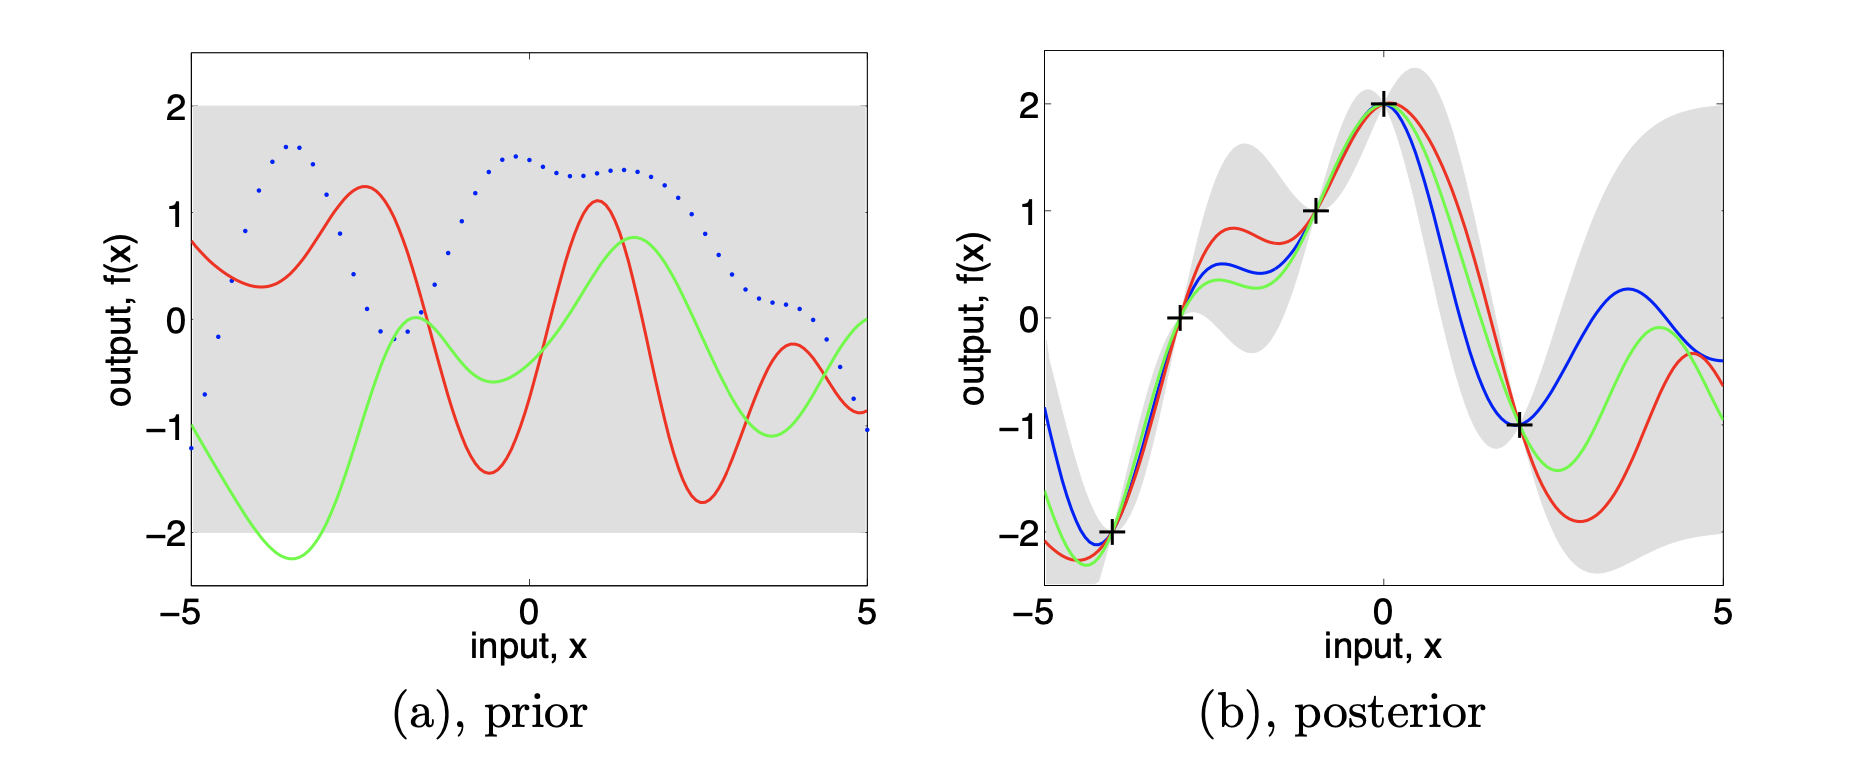
\includegraphics[width=0.90\textwidth]{img/gaussian_process.png}
\end{figure}
\newpage
In the example in Figure 5.1 the input values were equidistant, but this need not be the case. Notice that “informally” the functions look smooth. In fact the squared exponential covariance function is infinitely differentiable, leading to the process being infinitely mean-square differentiable. We also see that the functions seem to have a characteristic length-scale,
which informally can be thought as roughly the distance you have to move in input space before the function value can change significantly.\\
For Eq.5.1 the characteristic length-scale is around one unit. By replacing $|\boldsymbol{x}_p, \boldsymbol{x}_q|$ by $|\boldsymbol{x}_p, \boldsymbol{x}_q|/l$ for some positive constant $l$ we could change the characteristic length-scale of the process. Also, the overall variance of the random function can be controlled by a positive pre-factor before the $\exp$ in Eq.5.1.
\subsection{Prediction with Noise-free Observations}
We are usually not primarily interested in drawing random functions from the prior, but want to incorporate the knowledge that the training data provides about the function. Initially, we will consider the simple special case where the observations are noise free, that is we know $\{(\boldsymbol{x}_i, f_i)|i = 1,...,n\}$. The joint distribution of the training outputs, $\textbf{f}$, and the test outputs $\textbf{f}_*$ according to the prior is
\begin{equation*}
    \begin{bmatrix*}[l]
\textbf{f}\\
\textbf{f}_*
\end{bmatrix*}
\sim \mathcal{N}\Bigg(\boldsymbol{0}, \begin{bmatrix*}
K(X, X) & K(X, X_*)\\
K(X_*, X) & K(X_*, X_*)
\end{bmatrix*}\Bigg)
\end{equation*}
If there are $n$ training points and $n_*$ test points then $K(X, X_*)$ denotes the $n\times n_*$ matrix of the covariance evaluated at all pairs of training and test points, and similarly for the other entries.\\
To get the posterior distribution over functions we need to restrict this joint prior distribution to contain only those functions which agree with the observed data points. Graphically in Figure 5.1 you may think of generating functions from the prior, and rejecting the ones that disagree with the observations, although this strategy would not be computationally very efficient. Fortunately, in probabilistic terms this operation is extremely simple, corresponding to \textit{conditioning} the joint Gaussian prior distribution on the observations to give
\begin{equation}
    \textbf{f}_*|X_*,X, \textbf{f} \hspace{3pt}\sim \mathcal{N}(K(X_*, X)K(X, X)^{-1}\textbf{f},\hspace{3pt} K(X_*, X_*) - K(X_*, X)K(X, X)^{-1}K(X, X_*))
\end{equation}
Function values $\textbf{f}_*$ (corresponding to test inputs $X_*$) can be sampled from the joint posterior distribution by evaluating the mean and covariance matrix from Eq.5.2.\\
Figure 5.1(b) shows the results of these computations given the five data points marked with $+$ symbols. Notice that it is trivial to extend these computations to multidimensional inputs – one simply needs to change the evaluation of the covariance function in accordance with Eq.5.1, although the resulting functions may be harder to display graphically.
\subsection{Predicting using Noisy observations}
It is typical for more realistic modelling situations that we do not have access to function values themselves, but only noisy versions, i.e $y = f(\boldsymbol{x}) + \epsilon$. Assuming additive independent identically distributed Gaussian noise $\epsilon$ with variance $\sigma^2_n$, the prior on the noisy observations becomes
\begin{equation*}
    \text{cov}(y_p, y_q) = k(x_p, x_q) + \sigma^2_n\delta_{pq} \hspace{8pt}\text{or}\hspace{8pt} \text{cov}(\boldsymbol{y}) = K(X, X) + \sigma^2\mathds{1}
\end{equation*}
where $\delta_{pq}$ is a Kronecker delta which is one iff $p = q$ and zero otherwise. It follows from the independence assumption about noise, that a diagonal matrix is added, in comparison to the noise free case, Eq.5.1. Introducing the noise term we can write the joint distribution of the observed target values and the function values at the test locations under the prior as
\begin{equation*}
    \begin{bmatrix*}[l]
\boldsymbol{y}\\
\textbf{f}_*
\end{bmatrix*}
\sim \mathcal{N}\Bigg(\boldsymbol{0}, \begin{bmatrix*}
K(X, X) +  \sigma^2_n\mathds{1} & K(X, X_*)\\
K(X_*, X) & K(X_*, X_*)
\end{bmatrix*}\Bigg)
\end{equation*}
Deriving the conditional distribution corresponding to Eq.5.2 we arrive at the key predictive equations for Gaussian process regression
\begin{equation*}
    \textbf{f}_*|X,\textbf{y},X_* \sim \mathcal{N}(\overline{\textbf{f}}_*, \text{cov}(\textbf{f}_*)), \text{where}
\end{equation*}
\begin{equation}
    \overline{\textbf{f}}_* \triangleq \mathbb{E}[\textbf{f}_*|X, \boldsymbol{y}, X_*] = K(X_*, X)[K(X, X) + \sigma^2_N\mathds{1}]^{-1}\boldsymbol{y}
\end{equation}
\begin{equation}
    \text{cov}(\textbf{f}_*) = K(X_*, X_*) - K(X_*, X)[K(X, X) + \sigma^2_N\mathds{1}]^{-1}K(X, X_*)
\end{equation}\medskip

\textbf{Reminder}: Conditional Gaussian distribution
\begin{equation*}
    \begin{bmatrix*}[l]
\textbf{a}_1\\
\textbf{a}_2
\end{bmatrix*}
\sim \mathcal{N}\Bigg(\begin{bmatrix*}[l]
\boldsymbol{\mu}_1\\
\boldsymbol{\mu}_2
\end{bmatrix*}, \begin{bmatrix*}
\Sigma_{11} & \Sigma_{12}\\
\Sigma_{21} & \Sigma_{22}
\end{bmatrix*}\Bigg)
\end{equation*}
Then,
\begin{equation*}
    \textbf{a}_2 | \textbf{a}_1 = \boldsymbol{z} \sim \mathcal{N}(\boldsymbol{\mu}_2 + \Sigma_{21}\Sigma_{11}^{-1}(\boldsymbol{z} - \boldsymbol{\mu}_1), \Sigma_{22} - \Sigma_{21}\Sigma_{11}^{-1}\Sigma_{12})
\end{equation*}\medskip

The expressions involving $K(X, X), K(X, X_*)$ and $K(X_*, X_*)$ etc. can look rather unwieldy, so we now introduce a compact form of the notation setting $K = K(X, X)$ and $K_* = K(X, X_*)$. In the case there is only one test point $\boldsymbol{x}_*$ we write $\boldsymbol{k}(\boldsymbol{x_*}) = \boldsymbol{k_*}$ to denote the vector of covariances between the test point and the $n$ training points. Using this compact notation and for a single test point $\boldsymbol{x}_*$, equations 5.3 and 5.4 reduce to
\begin{equation}
    \bar{f}_* = \boldsymbol{k}_*^\intercal(K + \sigma^2_n\mathds{1})^{-1}\boldsymbol{y}
\end{equation}
\begin{equation}
    \text{Var}[f_*] = k(\boldsymbol{x}_*, \boldsymbol{x}_*) - \boldsymbol{k}_*^\intercal(K + \sigma^2_n\mathds{1})^{-1}\boldsymbol{k}_*
\end{equation}
Let us examine the predictive distribution given by equations 5.5 and 5.6. Note first that the mean prediction Eq.5.5 is a linear combination of observations $\boldsymbol{y}$; this is sometimes referred to as a \textit{linear predictor}. Another way to look at this equation is to see it as a linear combination of $n$ kernel functions, each one centered on a training point, by writing
\begin{equation}
    \bar{f}(\boldsymbol{x}_*) = \sum\limits_{i = 1}^{n} \alpha_i k(\boldsymbol{x}_i, \boldsymbol{x}_*)
\end{equation}
where $\boldsymbol{\alpha} = (K + \sigma^2_n\mathds{1})^{-1}\boldsymbol{y}$.\\
The fact that the mean prediction for $f(\boldsymbol{x}_*)$ can be written as Eq.5.7 despite the fact that the GP can be represented in terms of a (possible infinite) number of basis functions is one manifestation of the \textit{representer theorem}. We can understand this result intuitively because although the GP defines a joint Gaussian distribution over all of the $y$ variables.\\
For making predictions at $\boldsymbol{x}_*$ we only care about the $(n + 1)$-dimensional distribution defined by the $n$ training points and the test point. As a Gaussian distribution is marginalized by just taking the relevant block of joint covariance matrix it is clear that conditioning this $(n + 1)$-dimensional distribution on the observations gives us the desired result.\\
Note also that the variance in Eq.5.4 does not depend on the observed targets, but only on the inputs; this is a property of the Gaussian distribution. The variance is the difference between two terms; the first term $K(X_*, X_*)$ is simpy the prior covariance; from that is subtracted a (positive) term, representing the information the observations give us about the function. We can very simply compute the predictive distribution of test targets $\boldsymbol{y}_*$ by adding $\sigma^2_n\mathds{1}$ to the variance in the expression for cov($\textbf{f}_*$).\medskip

The predictive distribution for the GP model gives more than just pointwise errorbars of the simplified Eq.5.6. Although not stated explicitly, Eq.5.4 holds unchanged when $X_*$ denotes multiple test inputs; in this case the covariance of the test targets are computed (whose diagonal elements are the pointwise variances). In fact, Eq.5.3 is the mean function and Eq.5.4 the covariance function of the (Gaussian) posterior process.
\newpage
\begin{figure}[ht]
\caption{Algorithm 2.1: Predictions and log marginal likelihood for Gaussian process regression. The implementation addresses the matrix inversion required by equations 5.5 and 5.6 using Cholesky factorization. For multiple test cases lines 4-6 are repeated. The log determinant required in Eq.5.8 is computed from the Cholesky factor (for large $n$ it may not be possible to represent the determinant itself). The computational complexity is $n^3/6$ for the Cholesky decomposition in line 2, and $n^2/2$ for solving triangular systems in line 3 and (for each test case) in line 5.}
\centering
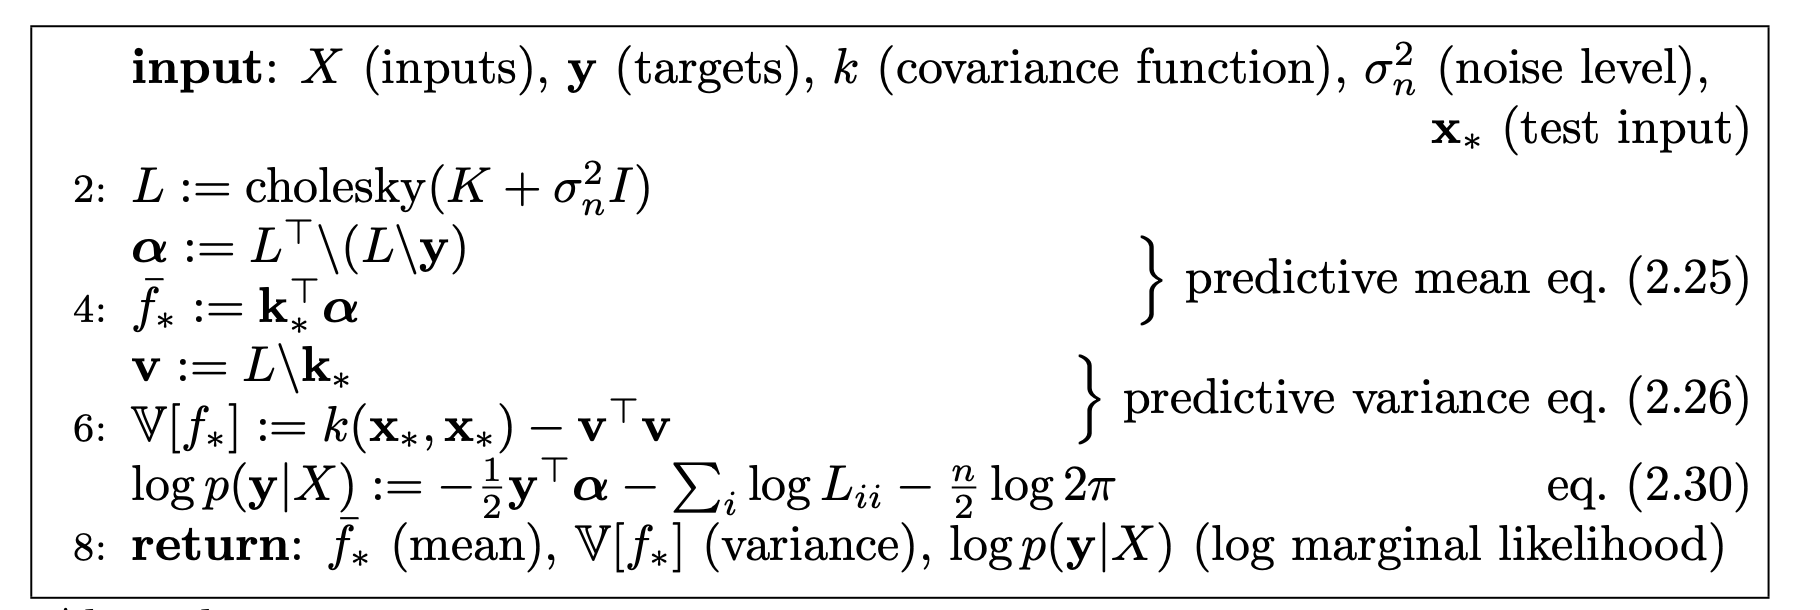
\includegraphics[width=0.90\textwidth]{img/algo_gp.png}
\end{figure}
The \textit{marginal likelihood}(or evidence) $p(\boldsymbol{y}|X)$ is the integral of the likelihood times the prior
\begin{equation*}
    p(\boldsymbol{y}|X) = \int p(\boldsymbol{y}|\textbf{f},X)p(\textbf{f}|X)d\textbf{f}
\end{equation*}
The term marginal likelihood refers to the marginalization over the function values \textbf{f}. Under the Gaussian process model the prior is Gaussian, $\textbf{f}|X \sim \mathcal{\boldsymbol{0}, K}$, or
\begin{equation}
    \log p(\boldsymbol{y}|X) = -\frac{1}{2}\boldsymbol{y}^\intercal(K + \sigma^2_n\mathds{1})^{-1}\boldsymbol{y} -\frac{1}{2}\log|K + \sigma^2_n\mathds{1}| -\frac{n}{2}\log2\pi
\end{equation}
This result can also be obtained directly by observing that $\boldsymbol{y} \sim \mathcal{N}(\boldsymbol{0}, K + \sigma^2_n\mathds{1})$.\medskip

A practical implementation of Gaussian process regression (GPR) is shown in Algorithm 2.1. The algorithm uses Cholesky decomposition, instead of directly inverting the matrix, since it is faster and numerically more stable. The algorithm returns the predictive mean and variance for noise free test data—to compute the predictive distribution for noisy test data $\boldsymbol{y}_*$, simply add the noise variance $    \sigma^2_n$ to the predictive variance of $f_*$.
\end{document}